\documentclass[upIatex,dvipdfmx,a4paper]{jsarticle}
\usepackage[utf8]{inputenc}
\usepackage{amsmath}
\usepackage{listings}
\usepackage[dvipdfmx]{graphicx}
\usepackage{float}
\usepackage{comment}
\usepackage{url}
\usepackage{multirow}
\usepackage{booktabs}
% ここからテンプレート設定
\usepackage{hyperref}
\usepackage{caption}
\usepackage{subcaption}
\usepackage{geometry}
\usepackage{longtable}
\geometry{left=25mm,right=25mm,top=30mm,bottom=30mm}

% listings の設定(ソースコード表示)
\lstset{
    basicstyle=\ttfamily\small,
    breaklines=true,
    numbers=left,
    numberstyle=\tiny,
    frame=single,
    captionpos=b,
    columns=fullflexible,
    escapeinside={(*@}{@*)},
    language=[LaTeX]TeX
}

% ドキュメント情報
\title{メディア情報学実験・メディア生成実験・最終レポート}
\author{2311084 久田友夢 k2311084@gl.cc.uec.ac.jp}
\date{\today}
% ここまでテンプレート設定

\begin{document}

\maketitle

\begin{abstract}
後で書く
\end{abstract}

\tableofcontents
\clearpage

\section{概要}
今回は、OpenGLを用いて、ゲームDead by Daylightの世界をミニチュア化したワールドを作成した。
Dead by Daylightは、4人の生存者と1人の殺人鬼に分かれて戦う非対称型対戦ゲームである。
生存者は、マップ上に点在する発電機を修理し、脱出ゲートを開けて脱出することが目的であり、殺人鬼は、生存者を捕まえてフックに吊るすことが目的である。
今回ミニチュア化した世界では、dbdにありそうな構造で作ったマップに板を配置した。
さらに一部のオブジェクトは、モデリングソフトを用いてモデリングした。
さらにオブジェクトの一部はtextureを貼り付けた。

作品タイトルは「Dead by Daylight Miniature World」とする。

マップとして次の構造で作成した。
\begin{figure}[H]
    \centering
    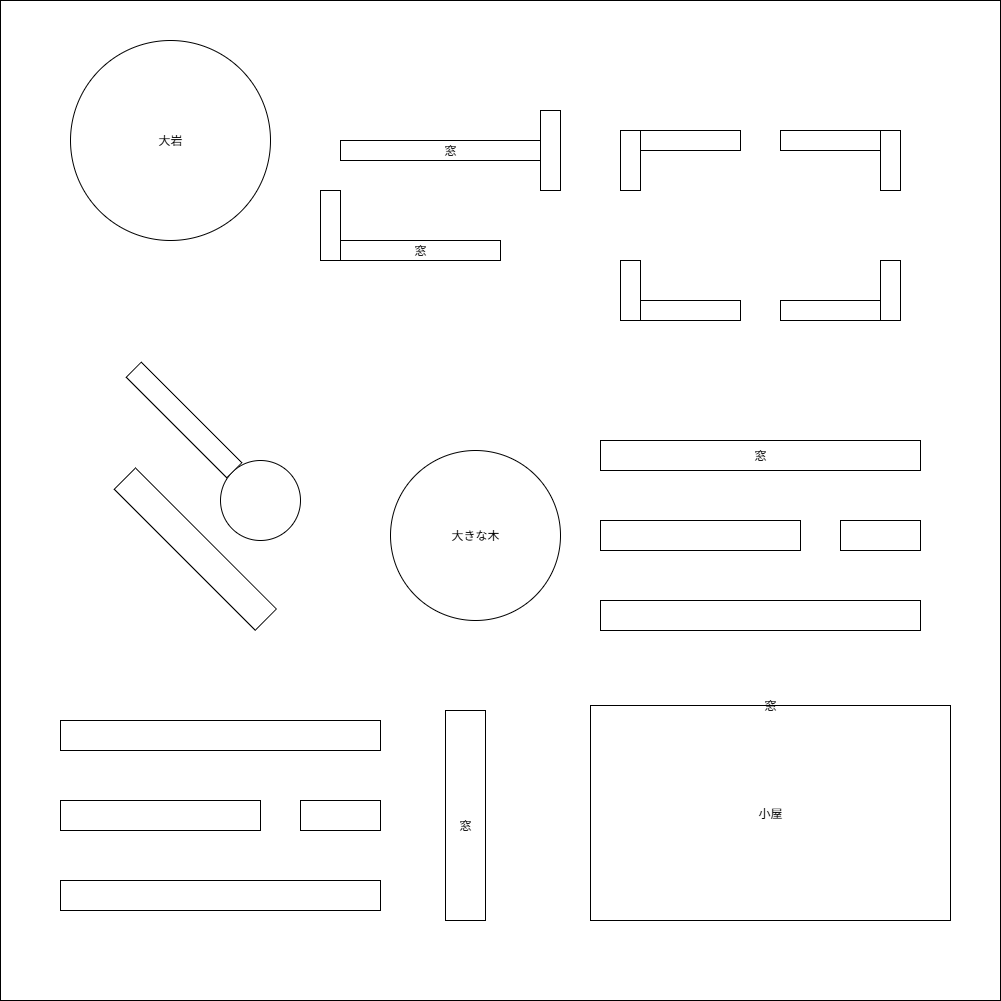
\includegraphics[width=10cm]{MediaEX_試案.png}
    \caption{マップの構造}
    \label{fig:my_label}
\end{figure}


\section{実行結果}
初めに実行結果を示す。
\begin{figure}[H]
    \centering
    \begin{subfigure}[b]{0.48\linewidth}
        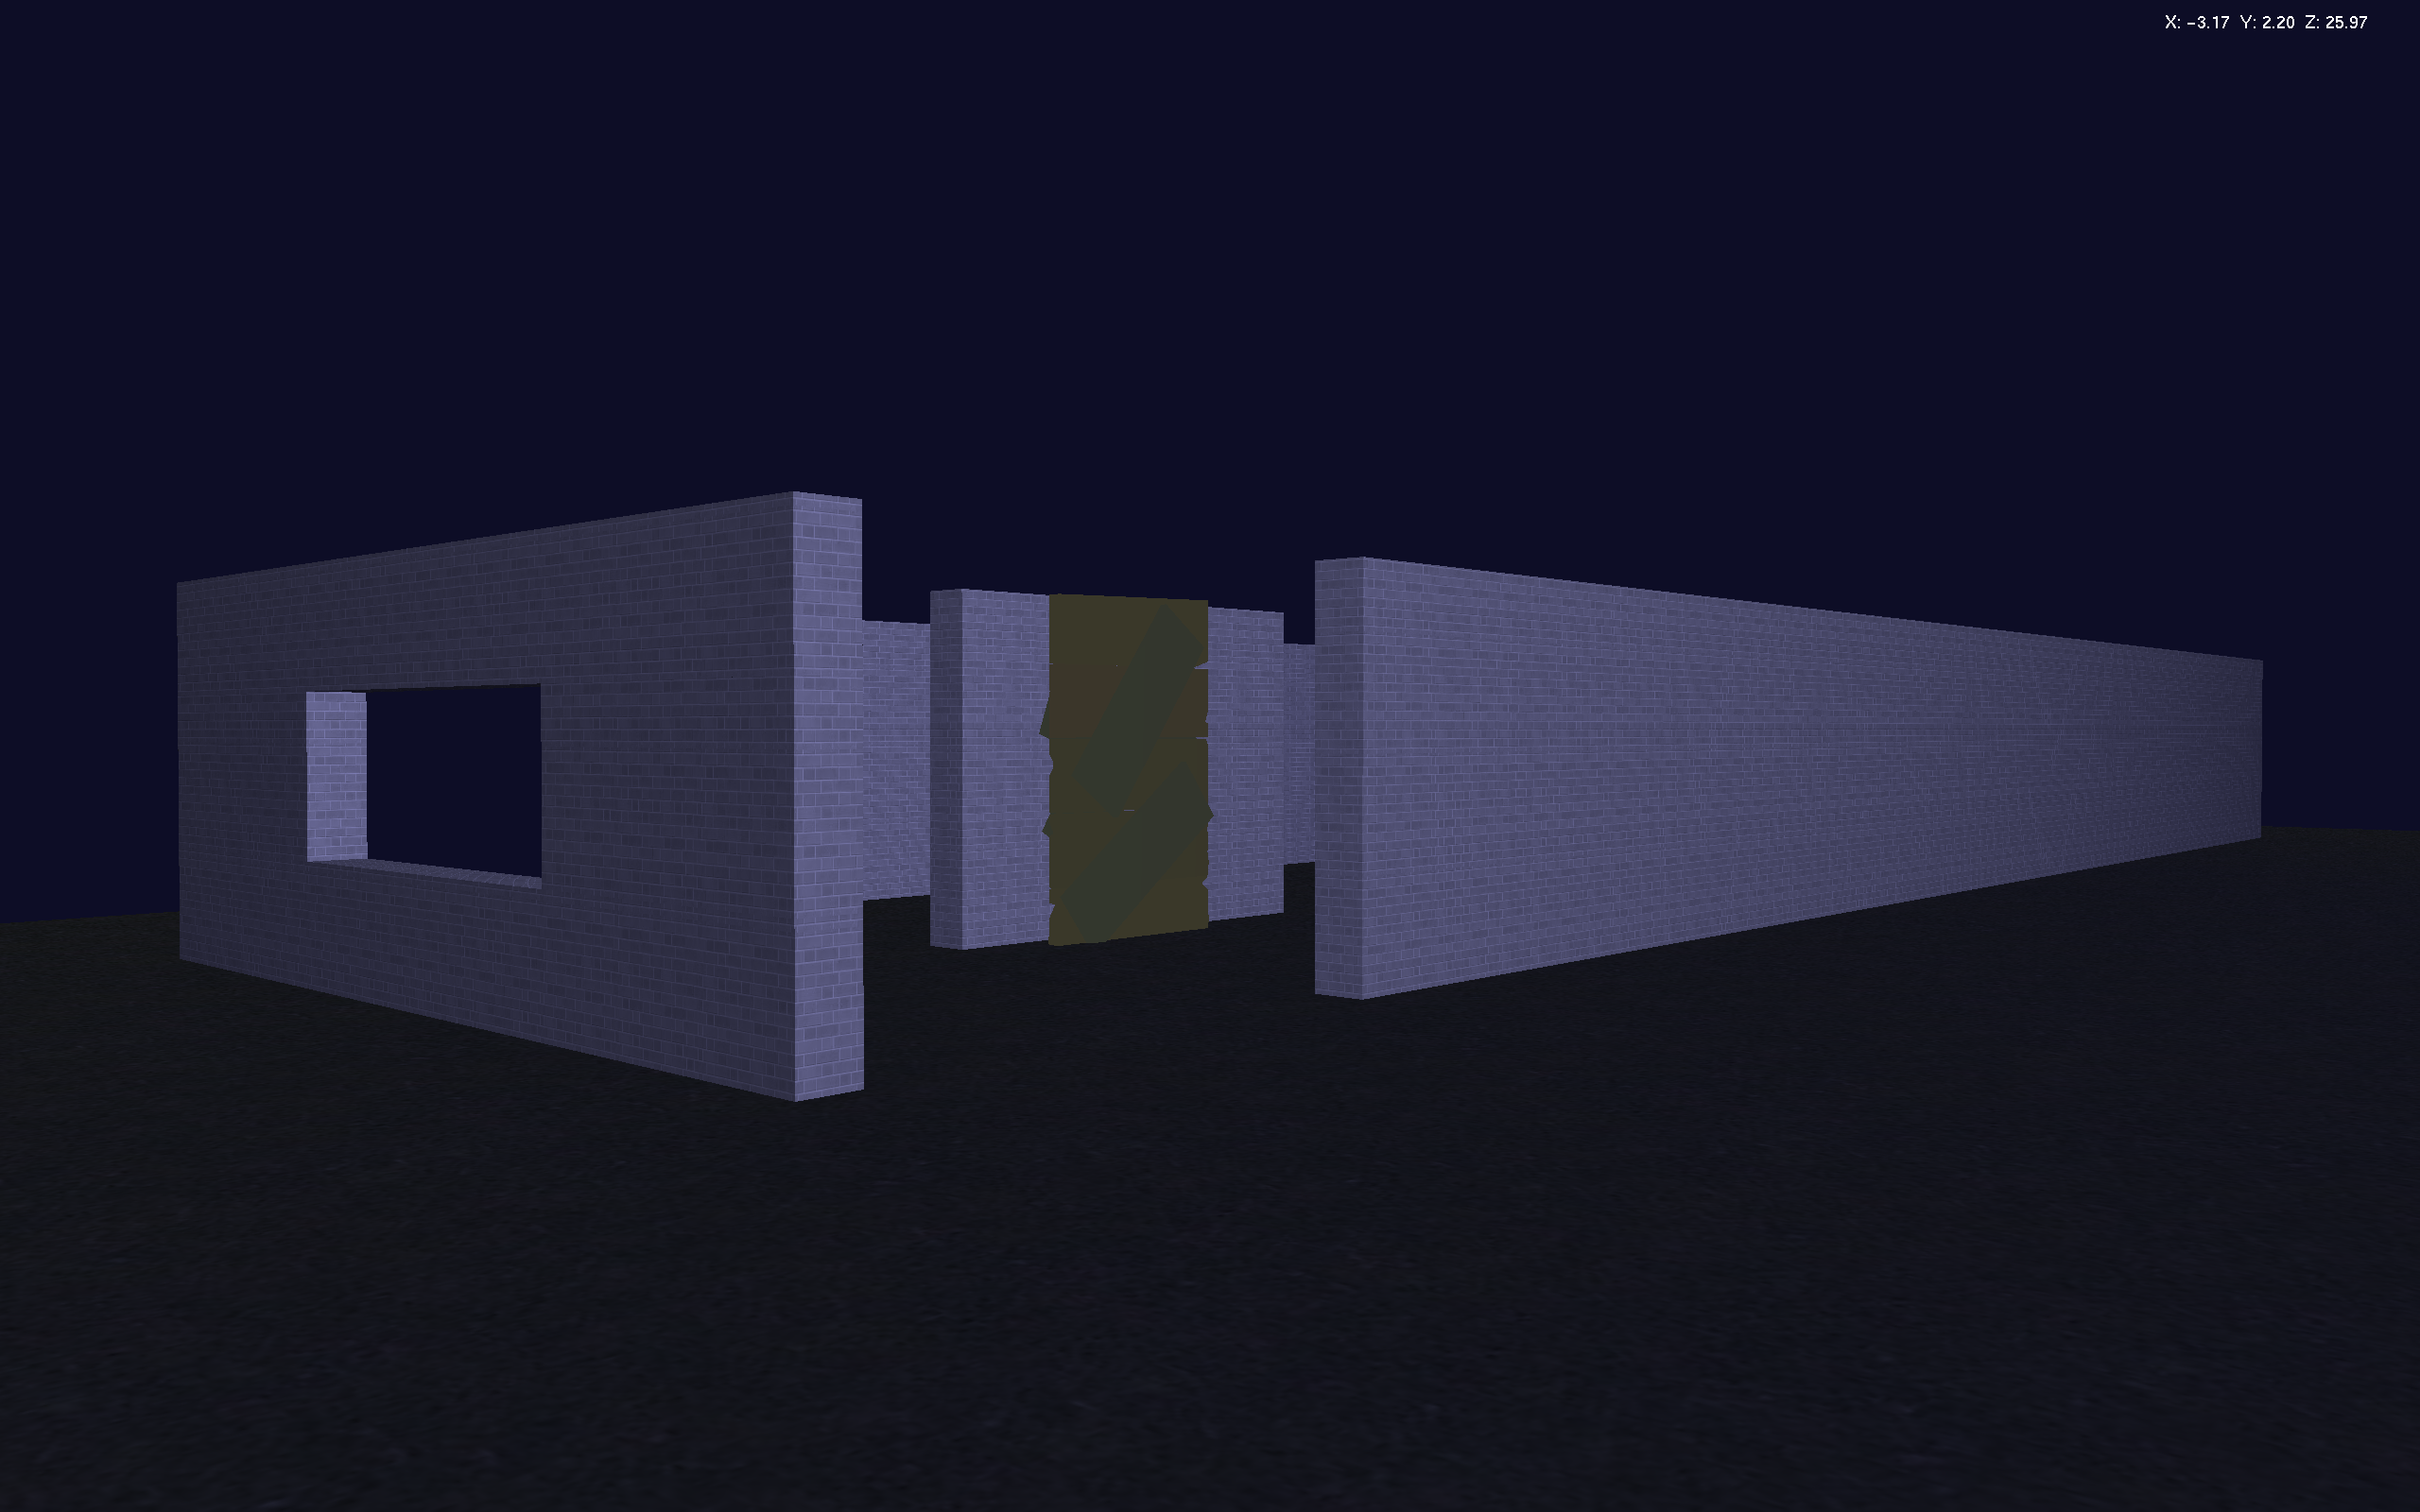
\includegraphics[width=\linewidth]{result1.png}
        \caption{壁とパレット}
        \label{fig:result1}
    \end{subfigure}
    \hfill
    \begin{subfigure}[b]{0.48\linewidth}
        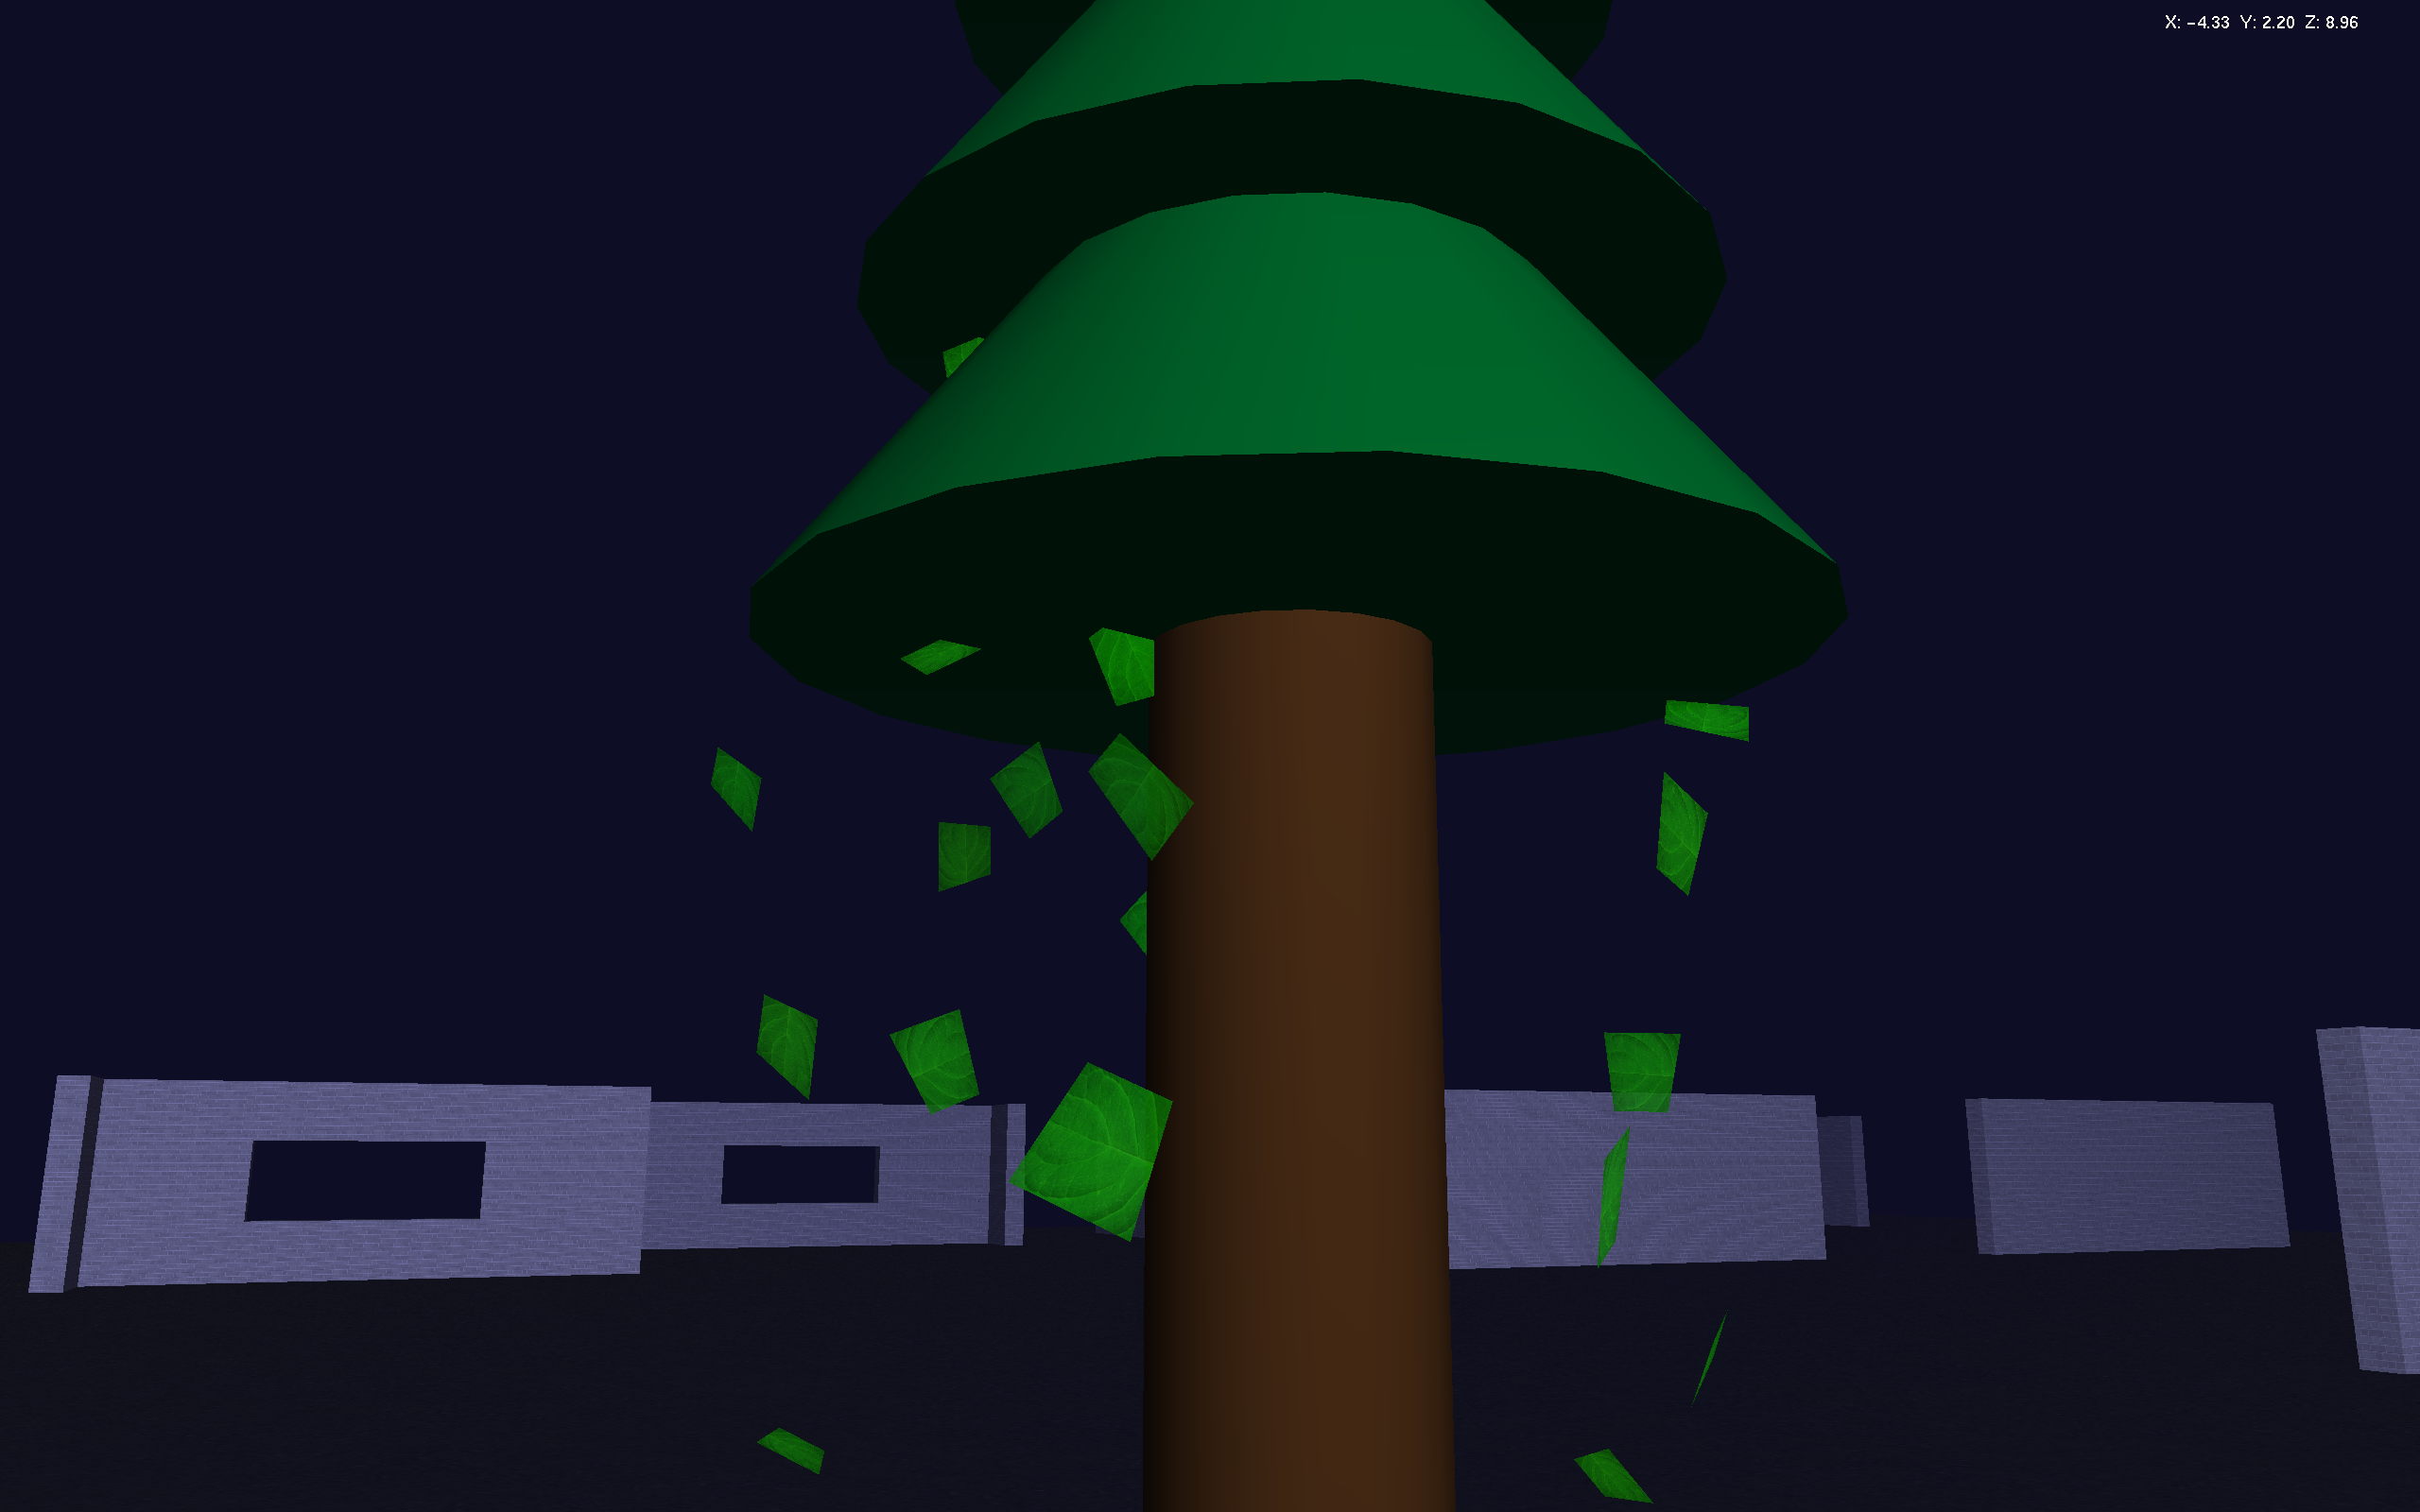
\includegraphics[width=\linewidth]{result2.png}
        \caption{近づくと葉っぱが落ちてくる木}
        \label{fig:result2}
    \end{subfigure}

    \vspace{4mm}

    \begin{subfigure}[b]{0.48\linewidth}
        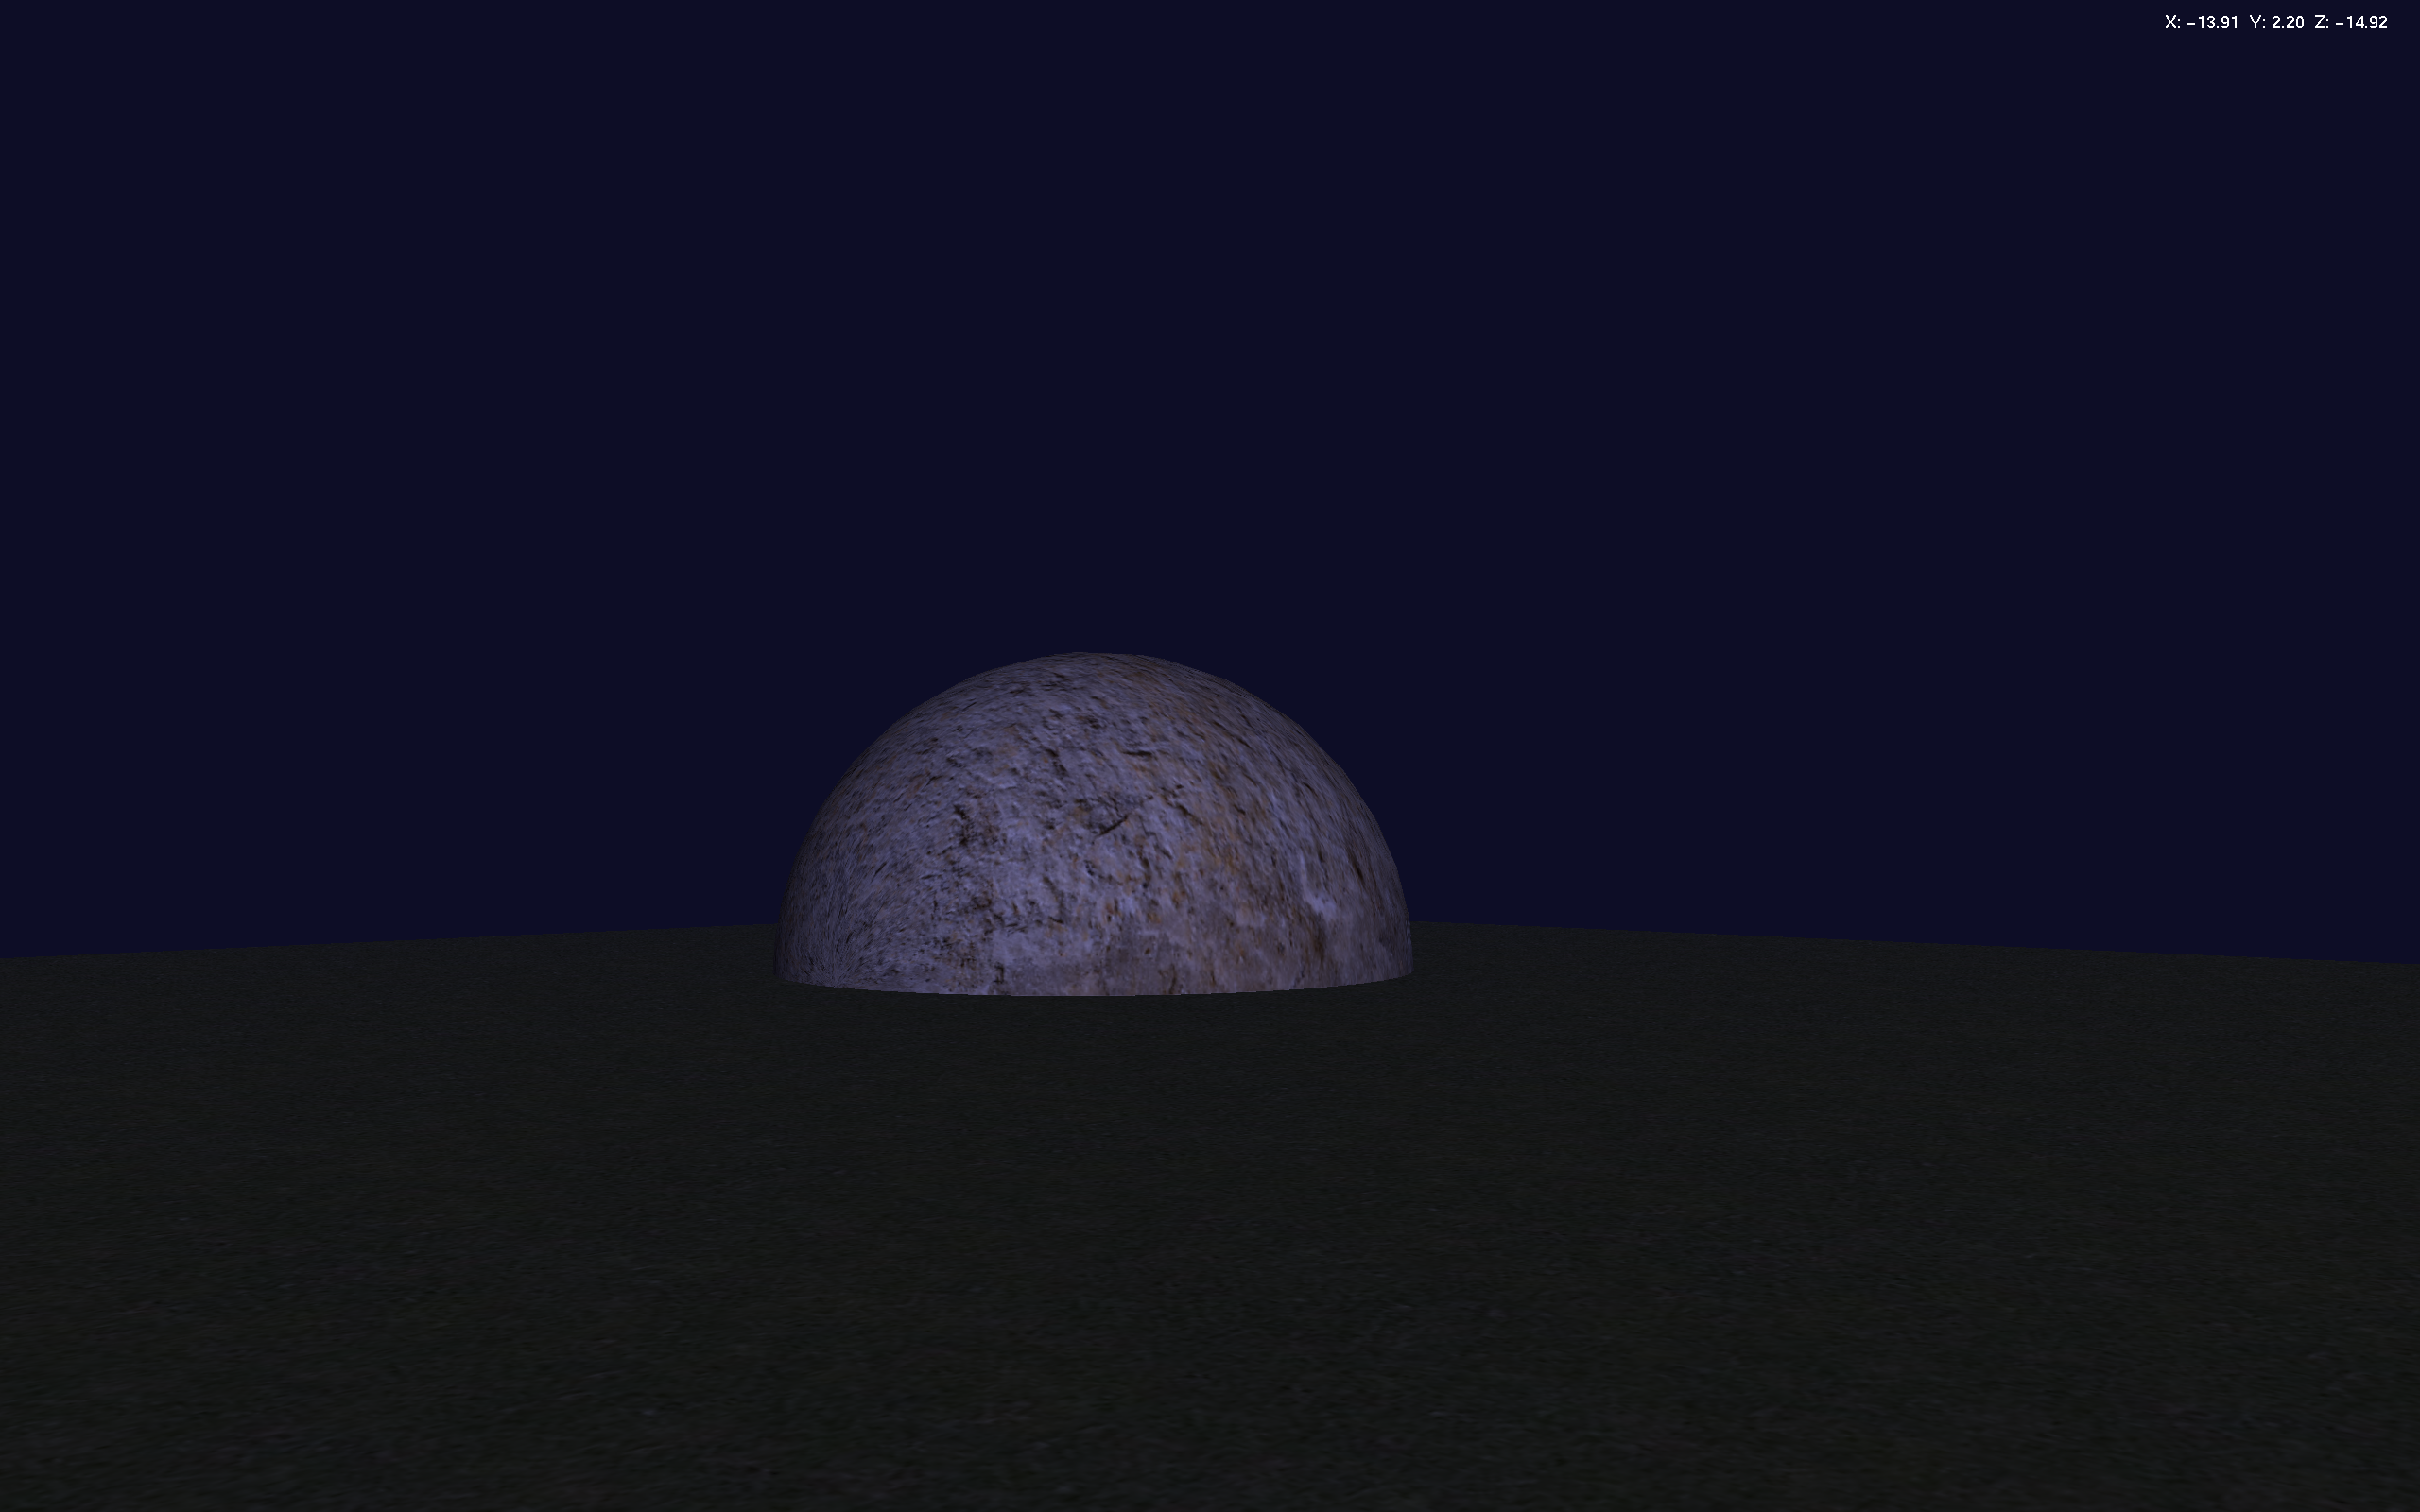
\includegraphics[width=\linewidth]{result3.png}
        \caption{tectureを貼り付けた岩}
        \label{fig:result3}
    \end{subfigure}
    \hfill
    \begin{subfigure}[b]{0.48\linewidth}
        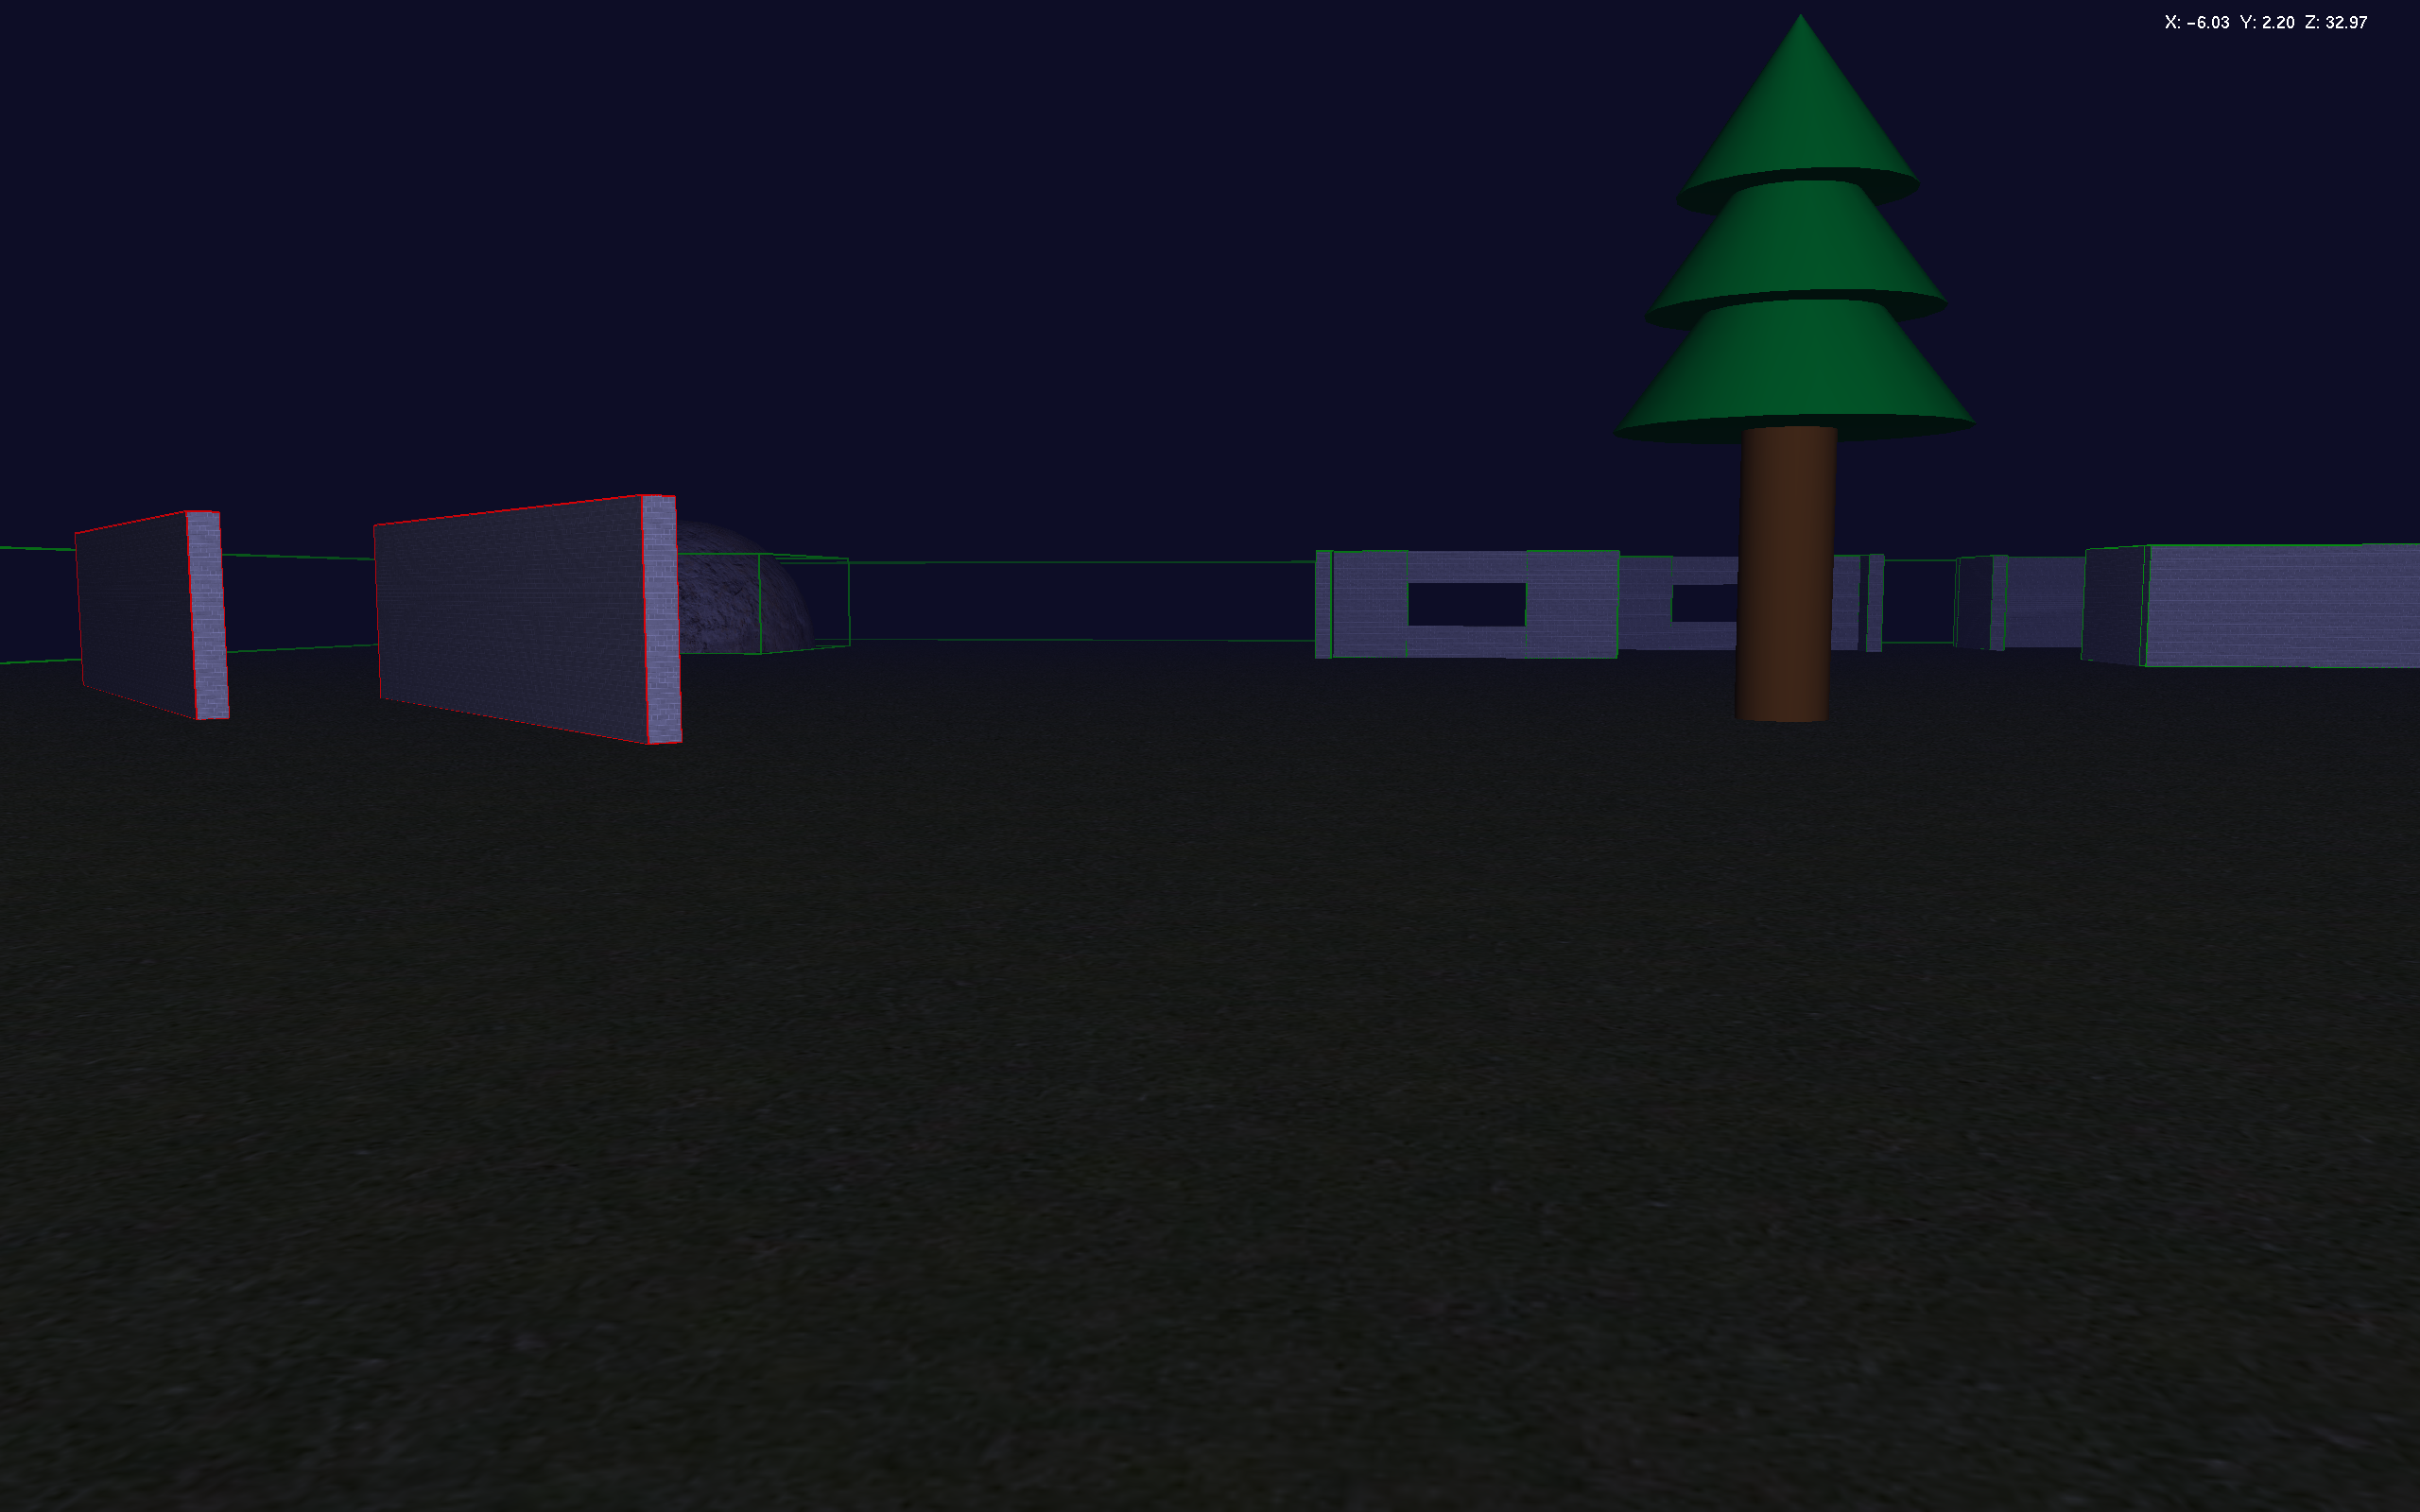
\includegraphics[width=\linewidth]{result4.png}
        \caption{当たり判定の可視化}
        \label{fig:result4}
    \end{subfigure}

    \caption{実行結果(result1〜result4)}
    \label{fig:results}
\end{figure}

\section{コード内容}
\subsection{ヘッダーファイル}
今回読み込んでいるヘッダーファイルは次のとおりである。
\begin{table}[H]
    \centering
    \caption{C++ヘッダファイルと本プログラムにおける用途}
    \label{tab:cpp_headers_intent}
    \begin{tabular}{lp{10cm}}
    \toprule
    \textbf{ヘッダーファイル/マクロ} & \textbf{このプログラムにおける用途} \\
    \midrule
    \texttt{<GL/glut.h>} & \textbf{実験での指定}。ウィンドウの表示、キーボード・マウス入力の受付、描画ループの管理など、アプリケーションの骨格として使用。 \\ \addlinespace

    \texttt{\#define \_USE\_MATH\_DEFINES} & カメラの向きや円運動の計算に必要な円周率の定数 \texttt{M\_PI} を \texttt{<cmath>} 内で有効化するために記述。 \\ \addlinespace

    \texttt{<cmath>} & カメラの向き(三角関数 \texttt{sin}, \texttt{cos})、当たり判定(平方根 \texttt{sqrt})、パーリンノイズ(\texttt{floor})など、3D空間の計算処理全般で使用。 \\ \addlinespace

    \texttt{<vector>} & 壁、パレット、落ち葉など、シーン内に複数存在するオブジェクトのリストを可変長配列として管理するために使用。 \\ \addlinespace

    \texttt{<cstdio>} & \texttt{sprintf} を使い、プレイヤーの現在座標をリアルタイムで文字列に変換し、画面右上のHUDに表示するために使用。 \\ \addlinespace

    \texttt{<cctype>} & \texttt{tolower} を使い、キーボード入力で大文字・小文字を区別せず(例:'W'と'w'を同じ前進命令として)扱うために使用。 \\ \addlinespace

    \texttt{<opencv2/opencv.hpp>} & 地面や壁、岩などに貼り付けるテクスチャ(.jpg画像)をファイルから読み込み、OpenGLで扱える形式に変換するために使用。 \\ \addlinespace

    \texttt{<iostream>} & モデルやテクスチャの読み込みが成功したか、あるいは失敗したかといったプログラムの動作状況をコンソールに出力するために使用。 \\ \addlinespace

    \texttt{<string>} & \texttt{".obj"} や \texttt{".jpg"} ファイルのパスを文字列として扱い、モデルやテクスチャの読み込み関数に渡すために使用。 \\ \addlinespace

    \texttt{<locale.h>} & PCの地域設定に依らず、.objファイル内の小数点を一貫して「.」として読み込ませ、モデルの読み込みエラーを防ぐために使用。 \\ \addlinespace

    \texttt{<random>} & 舞い散る葉の位置・色・回転速度などをランダムに決定し、自然に見えるパーティクルエフェクトを生成するために使用。 \\ \addlinespace

    \texttt{<algorithm>} & 地面に落ちた葉をリストから効率的に削除する(\texttt{std::remove\_if})ため、またパーリンノイズの初期化(\texttt{std::shuffle})のために使用。 \\ \addlinespace

    \texttt{<numeric>} & パーリンノイズの計算に必要な配列を \texttt{0, 1, 2...} という連番で高速に初期化するため(\texttt{std::iota})に使用。 \\ \addlinespace

    \texttt{<limits>} & 当たり判定の内部計算で、比較の初期値として浮動小数点数の最大値を取得するために使用。 \\ \addlinespace

    \texttt{<cstring>} & 自作の透視投影行列の計算関数内で、行列データを効率的にゼロで初期化するため(\texttt{memset})に使用。 \\ \addlinespace

    \texttt{"tiny\_obj\_loader.h"} & ステージに配置されているパレットと家の3Dモデル(.obj形式)をファイルから読み込み、描画可能なデータに変換するために使用。 \\
    \bottomrule
    \end{tabular}
\end{table}
\subsection{グローバル変数}
\begin{table}[H]
    \centering
    \caption{グローバル変数の役割}
    \label{tab:global_variables}
    \begin{tabular}{p{4cm}p{4cm}p{8cm}}
        \toprule
        \textbf{型} & \textbf{変数名} & \textbf{目的} \\
        \midrule
        \multicolumn{3}{l}{\textit{--- カメラ・プレイヤー関連 ---}} \\
        \texttt{float} & \texttt{cameraX, cameraY, cameraZ} & プレイヤー(カメラ)の現在位置(X, Y, Z座標)を保持する。 \\
        \texttt{float} & \texttt{yaw, pitch} & プレイヤーの視点の向き(水平方向・垂直方向の回転角度)を保持する。 \\
        \texttt{int} & \texttt{lastMouseX, lastMouseY} & マウス視点操作で、前フレームのマウスカーソル位置を記憶するために使用。 \\
        \texttt{bool} & \texttt{firstMouse} & マウスがウィンドウに入った直後の視点移動の急なブレを防ぐためのフラグ。 \\
        \texttt{bool} & \texttt{justWarped} & マウスカーソルを画面中央に強制移動させた直後かを判定するフラグ。 \\
        \texttt{bool} & \texttt{isMouseLookActive} & マウスカーソルがウィンドウ内にあるときだけ視点操作を有効にするためのフラグ。 \\
        \addlinespace
        \multicolumn{3}{l}{\textit{--- ウィンドウ・シーン関連 ---}} \\
        \texttt{int} & \texttt{windowWidth, windowHeight} & ウィンドウの現在の幅と高さを保持し、描画範囲の調整に使用。 \\
        \texttt{bool} & \texttt{keyStates[256]} & 全てのキー(256文字分)の押下状態(押されている/いない)を管理する配列。 \\
        \texttt{bool} & \texttt{showColliders} & デバッグ用に当たり判定のワイヤーフレーム表示を切り替えるためのフラグ。 \\
        \texttt{GLuint} & \texttt{...TextureID} & OpenGLで管理される各テクスチャ(地面、壁など)の識別番号を保持する。 \\
        \texttt{float} & \texttt{g\_time} & プログラム開始からの経過時間を保持し、アニメーションの同期に使用。 \\
        \addlinespace
        \multicolumn{3}{l}{\textit{--- オブジェクト・当たり判定関連 ---}} \\
        \texttt{Model} & \texttt{paletModel, blenderModel} & tinyobjloaderで読み込んだ3Dモデルの頂点や材質データを保持する。 \\
        \texttt{vector<BoundingBox>} & \texttt{wallColliders} & 壁などの動かないオブジェクトの当たり判定(AABB)情報をリストで管理。 \\
        \texttt{vector<OBB>} & \texttt{obbColliders} & 回転を考慮する必要があるオブジェクトの当たり判定(OBB)情報をリストで管理。 \\
        \texttt{vector<Pallet>} & \texttt{pallets} & シーン内に存在する全パレットの位置、回転、状態などをリストで管理。 \\
        \texttt{vector<Leaf>} & \texttt{fallingLeaves} & 画面内に表示されている全ての葉パーティクルの状態をリストで管理。 \\
        \bottomrule
    \end{tabular}
\end{table}
\subsection{関数}
\subsubsection{関数一覧}
はじめに今回作成した関数の概要をまとめる。
\begin{longtable}{lp{0.7\textwidth}} % 説明欄の横幅をテキスト幅の70%に修正
    \caption{関数とその目的}
    \label{tab:functions_long} \\

    \toprule
    \textbf{関数名} & \textbf{目的} \\
    \midrule
    \endfirsthead

    \multicolumn{2}{l}{\tablename~\thetable{} -- 前ページからの続き} \\
    \toprule
    \textbf{関数名} & \textbf{目的} \\
    \midrule
    \endhead

    \bottomrule
    \endlastfoot

    % --- 表の内容 ---
    \multicolumn{2}{l}{\textit{--- 数学ヘルパー関数 ---}} \\
    \texttt{cross()} & 3Dベクトルの外積を計算する。カメラの向きの計算で使用。 \\
    \texttt{dot()} & 3D/2Dベクトルの内積を計算する。当たり判定やカメラ計算で使用。 \\
    \texttt{normalize()} & 3Dベクトルの長さを1に正規化する。カメラの向きの計算で使用。 \\
    \texttt{perspectiveMatrix()} & 透視投影行列を自前で作成する。 \\
    \texttt{lookAtMatrix()} & カメラの位置と注視点からビュー行列を自前で作成する。 \\
    \texttt{drawTexturedSphere()} & テクスチャ付きの球体を自前で描画する。 \\
    \addlinespace
    \multicolumn{2}{l}{\textit{--- パーリンノイズ関連関数 ---}} \\
    \texttt{fade(), linearInterpolate(), grad()} & パーリンノイズの値を滑らかに補間するための計算用ヘルパー関数。 \\
    \texttt{initPerlinNoise()} & パーリンノイズ生成に必要なランダムな変換テーブルを最初に一度だけ作成する。 \\
    \texttt{perlinNoise()} & 指定された3次元座標に対応するノイズ値を生成し、葉の揺らぎに使用。 \\
    \addlinespace
    \multicolumn{2}{l}{\textit{--- モデル・テクスチャ処理関数 ---}} \\
    \texttt{calculateModelBBox()} & .objモデルの全頂点を調査し、モデルを囲む最小の箱(バウンディングボックス)を計算。 \\
    \texttt{loadObjModel()} & tinyobjloaderを使い、.obj形式の3Dモデルファイルを読み込んでデータ構造に格納する。 \\
    \texttt{drawObjModel()} & 読み込んだ3Dモデルを指定された設定で描画する。発光効果にも対応。 \\
    \texttt{loadTexture()} & OpenCVを使い、画像ファイルを読み込んでOpenGLのテクスチャとして利用可能にする。 \\
    \addlinespace
    \multicolumn{2}{l}{\textit{--- 描画関連関数 ---}} \\
    \texttt{renderBitmapString()} & 画面上の指定座標にデバッグ情報などの文字列を描画する。 \\
    \texttt{drawHUD()} & 画面右上にプレイヤーの現在座標をオーバーレイ表示する。 \\
    \texttt{drawGround(), etc.} & 地面、壁、木、岩など、ステージを構成する各要素を描画する。 \\
    \texttt{drawCylinder()} & 木の幹などを描画するために使用する円柱の描画関数。 \\
    \texttt{drawFallingLeaves()} & 葉のパーティクルエフェクトを描画する。 \\
    \texttt{drawColliders()} & デバッグ用に当たり判定領域をワイヤーフレームで可視化する。 \\
    \addlinespace
    \multicolumn{2}{l}{\textit{--- 初期化・状態更新関数 ---}} \\
    \texttt{setupColliders()} & 壁やオブジェクトの当たり判定をプログラム開始時にセットアップする。 \\
    \texttt{setupPallets()} & パレットオブジェクトを初期位置に配置する。 \\
    \texttt{updatePallets()} & パレットの浮遊アニメーションやインタラクション後の状態を更新する。 \\
    \texttt{spawnLeaf()} & 新しい葉パーティクルをランダムな設定で生成する。 \\
    \texttt{updateFallingLeaves()} & 全ての葉パーティクルの状態をフレーム毎に更新し、不要なものを消去する。 \\
    \texttt{check...Collision()} & プレイヤーと各オブジェクトとの当たり判定を計算し、衝突解決を行う。 \\
    \addlinespace
    \multicolumn{2}{l}{\textit{--- GLUTコールバック関数 ---}} \\
    \texttt{display()} & 画面の再描画時に呼び出され、全ての描画命令を発行するメイン描画関数。 \\
    \texttt{update()} & 一定時間ごとに呼び出され、プレイヤーの位置、アニメーションなどゲーム全体のロジックを更新。 \\
    \texttt{keyboard(), keyboardUp()} & キーの押下・解放を検知し、プレイヤーの移動や機能のON/OFFを行う。 \\
    \texttt{mouseMotion()} & マウスの動きを検知し、プレイヤーの視点移動に反映させる。 \\
    \texttt{reshape()} & ウィンドウサイズ変更時に呼び出され、描画のアスペクト比などを再設定する。 \\
    \texttt{entry()} & マウスカーソルの出入りを検知し、視点操作の有効/無効を切り替える。 \\
    \texttt{initScene()} & プログラム起動時に一度だけ呼び出され、シーン全体の初期設定を行う。 \\
    \addlinespace
    \multicolumn{2}{l}{\textit{--- メイン関数 ---}} \\
    \texttt{main()} & プログラムのエントリーポイント。GLUTの初期化とウィンドウ作成、コールバック関数の登録を行う。 \\
\end{longtable}

ここから1つ1つの関数について説明を行う。
\subsubsection{cross()}
\begin{lstlisting}[language=C++, caption={cross() 関数}, label={lst:cross}]
/**
 * @brief 2つの3Dベクトルの外積を計算する。
 * @param a 1つ目のベクトル
 * @param b 2つ目のベクトル
 * @return 2つのベクトルの外積ベクトル
 */
Vec3 cross(const Vec3& a, const Vec3& b) {
    return {a.y * b.z - a.z * b.y, a.z * b.x - a.x * b.z, a.x * b.y - a.y * b.x};
}
\end{lstlisting}

この関数では、2つの3Dベクトルに対する外積を計算している。

特にlookAtMatrixというカメラ制御関数において右方向と上方向を決定するときに使用するヘルプ関数である。
例えば、カメラの正面の向きと上の向きの外積を計算することにより、右方向が決定できる。
\subsubsection{dot()}
\begin{lstlisting}[language=C++, caption={dot() 関数 (3Dベクトル版)}, label={lst:dot}]
/**
 * @brief 2つの3Dベクトルの内積を計算する。
 * @param a 1つ目のベクトル
 * @param b 2つ目のベクトル
 * @return 2つのベクトルの内積
 */
float dot(const Vec3& a, const Vec3& b) {
    return a.x * b.x + a.y * b.y + a.z * b.z;
}
\end{lstlisting}
この関数では、2つの3Dベクトルに対する内積を計算している。

このプログラムでは、ベクトルの長さを決めるときや、カメラの位置を決定するときにdot関数を使っている。

\subsubsection{normalize()}
\begin{lstlisting}[language=C++, caption={normalize() 関数}, label={lst:normalize}]
/**
 * @brief 3Dベクトルを正規化する(長さを1にする)。
 * @param v 正規化するベクトル
 * @return 正規化されたベクトル
 */
Vec3 normalize(const Vec3& v) {
    float len = std::sqrt(dot(v, v));
    if (len > 0) {
        return {v.x / len, v.y / len, v.z / len};
    }
    return v;
}
\end{lstlisting}

この関数はベクトルの正規化を行う関数である。
三平方の定理を用いてベクトルの長さを計算し、その結果で割っている。

この関数は、lookAtMatrix()の中で、カメラの向きを定義する軸ベクトルを単位ベクトルにそろえるために使用している。
\subsubsection{perspectiveMatrix}
\begin{lstlisting}[language=C++, caption={perspectiveMatrix() 関数}, label={lst:perspectiveMatrix}]
/**
 * @brief 透視投影行列を作成する。
 * @param mat 結果を格納する16要素のfloat配列
 * @param fovY Y方向の視野角 (度数法)
 * @param aspect アスペクト比 (幅 / 高さ)
 * @param zNear 前方クリッピング面までの距離
 * @param zFar 後方クリッピング面までの距離
 */
void perspectiveMatrix(float* mat, float fovY, float aspect, float zNear, float zFar) {
    memset(mat, 0, 16 * sizeof(float));
    float f = 1.0f / tanf(fovY * (M_PI / 180.0f) / 2.0f);
    mat[0] = f / aspect;
    mat[5] = f;
    mat[10] = (zFar + zNear) / (zNear - zFar);
    mat[11] = -1.0f;
    mat[14] = (2.0f * zFar * zNear) / (zNear - zFar);
}
\end{lstlisting}
この関数は3D空間を2Dの画面に映し出すための透視投影行列を作成するものである。

forYは視野角を、aspectはアスペクト比を。zNearとzForて描画範囲を設定している。

この関数はreshape()で使用している。特に視点移動で苦労した際に追加した。
現在はフルスクリーンを固定にしているため、実際に動くことは少ないが、フルスクリーン設定を解除したときにreshapeにてウィンドウサイズが変更されたときに呼び出される。
\subsubsection{lookAtMatrix()}
\begin{lstlisting}[language=C++, caption={lookAtMatrix() 関数}, label={lst:lookAtMatrix}]
/**
 * @brief ビュー行列を作成する。
 * @param mat 結果を格納する16要素のfloat配列
 * @param eye カメラの位置
 * @param center 注視点
 * @param up カメラの上方向
 */
void lookAtMatrix(float* mat, const Vec3& eye, const Vec3& center, const Vec3& up) {
    Vec3 f = normalize({center.x - eye.x, center.y - eye.y, center.z - eye.z});
    Vec3 s = normalize(cross(f, up));
    Vec3 u = cross(s, f);

    mat[0] = s.x;
    mat[4] = s.y;
    mat[8] = s.z;
    mat[12] = -dot(s, eye);

    mat[1] = u.x;
    mat[5] = u.y;
    mat[9] = u.z;
    mat[13] = -dot(u, eye);

    mat[2] = -f.x;
    mat[6] = -f.y;
    mat[10] = -f.z;
    mat[14] = dot(f, eye);

    mat[3] = 0.0f;
    mat[7] = 0.0f;
    mat[11] = 0.0f;
    mat[15] = 1.0f;
}
\end{lstlisting}
この関数は、3D空間における仮想的なカメラの位置と向きを定義するための関数である。
今回の視点移動はカメラを動かすのではなく、3D空間全てのオブジェクトを動かすことで、あたかもカメラが移動しているかのように錯覚させて、実装している。

この関数はフレームごとの描画を行うdisplay()関数にて使用している。
\subsubsection{drawTextureSphere()}
\begin{lstlisting}[language=C++, caption={drawTexturedSphere() 関数}, label={lst:drawTexturedSphere}]
/**
 * @brief テクスチャマッピング可能な球体を描画する。
 * @param radius 球の半径
 * @param slices 経度方向の分割数
 * @param stacks 緯度方向の分割数
 */
void drawTexturedSphere(GLdouble radius, GLint slices, GLint stacks) {
    for (int i = 0; i < stacks; ++i) {
        GLdouble lat0 = M_PI * (-0.5 + (double)i / stacks);
        GLdouble z0 = radius * sin(lat0);
        GLdouble zr0 = radius * cos(lat0);
        GLdouble lat1 = M_PI * (-0.5 + (double)(i + 1) / stacks);
        GLdouble z1 = radius * sin(lat1);
        GLdouble zr1 = radius * cos(lat1);
        glBegin(GL_QUAD_STRIP);
        for (int j = 0; j <= slices; ++j) {
            GLdouble lng = 2 * M_PI * (double)j / slices;
            GLdouble x = cos(lng);
            GLdouble y = sin(lng);
            glNormal3d(x * zr1, y * zr1, z1);
            glTexCoord2d((double)j / slices, (double)(i + 1) / stacks);
            glVertex3d(x * zr1, y * zr1, z1);
            glNormal3d(x * zr0, y * zr0, z0);
            glTexCoord2d((double)j / slices, (double)i / stacks);
            glVertex3d(x * zr0, y * zr0, z0);
        }
        glEnd();
    }
}
\end{lstlisting}

この関数では、textureを貼り付けることができる3Dの球体を作成する。

特に大きな岩を作成するときに使用した。

\subsubsection{fade(),linearlnterpolate(),grad()}
\begin{lstlisting}[language=C++, caption={パーリンノイズ用ヘルパー関数}, label={lst:perlin_helpers}]
/**
 * @brief パーリンノイズで滑らかな補間を行うためのフェード関数。
 * @param t 入力値 (通常0.0~1.0)
 * @return 補間された値
 */
float fade(float t) { return t * t * t * (t * (t * 6 - 15) + 10); }

/**
 * @brief 線形補間を行う。
 * @param a 開始値
 * @param b 終了値
 * @param t 補間係数 (0.0~1.0)
 * @return 補間された値
 */
float linearInterpolate(float a, float b, float t) { return a + t * (b - a); }

/**
 * @brief ハッシュ値に基づいて勾配ベクトルを計算する。
 * @param hash ハッシュ値
 * @param x x座標
 * @param y y座標
 * @param z z座標
 * @return 勾配ベクトルの計算結果
 */
float grad(int hash, float x, float y, float z) {
    int h = hash & 15;
    float u = h < 8 ? x : y;
    float v = h < 4 ? y : (h == 12 || h == 14 ? x : z);
    return ((h & 1) == 0 ? u : -u) + ((h & 2) == 0 ? v : -v);
}
\end{lstlisting}
これらの関数群はparlinNoize()関数の実装のために作ったヘルパー関数である。

fade()はパーリンノイズにて滑らかな保管を行うための関数である。

linearInterpolate()は線形補完を行うための関数である。

grad()はハッシュ値に基づいて勾配ベクトルを計算するための関数である。

詳細はparlinNoise()にて説明する。

\subsubsection{initPerlinNoise()}
\begin{lstlisting}[language=C++, caption={initPerlinNoise() 関数}, label={lst:initPerlinNoise}]
/**
 * @brief パーリンノイズ生成器を初期化する。ランダムな置換テーブルを作成する。
 */
void initPerlinNoise() {
    std::iota(p, p + 256, 0);
    std::shuffle(p, p + 256, rng);
    for (int i = 0; i < 256; ++i) {
        p[i + 256] = p[i];
    }
}
\end{lstlisting}

この間数はパーリンノイズを作成するために不可欠な置換テーブルという乱数リストの作成を行うものである。

update()と並列処理をすると、この処理が重くカクカクしてしまったので、起動時に呼び出すようにした。

\subsubsection{perlinNoise()}
\begin{lstlisting}[language=C++, caption={perlinNoise() 関数}, label={lst:perlinNoise}]
/**
 * @brief 3次元パーリンノイズを生成する。
 * @param x x座標
 * @param y y座標
 * @param z z座標
 * @return 0.0から1.0の範囲のノイズ値
 */
float perlinNoise(float x, float y, float z) {
    int X = (int)floor(x) & 255;
    int Y = (int)floor(y) & 255;
    int Z = (int)floor(z) & 255;
    x -= floor(x);
    y -= floor(y);
    z -= floor(z);
    float u = fade(x), v = fade(y), w = fade(z);
    int A = p[X] + Y, AA = p[A] + Z, AB = p[A + 1] + Z;
    int B = p[X + 1] + Y, BA = p[B] + Z, BB = p[B + 1] + Z;
    float res = linearInterpolate(
        linearInterpolate(
            linearInterpolate(grad(p[AA], x, y, z), grad(p[BA], x - 1, y, z), u),
            linearInterpolate(grad(p[AB], x, y - 1, z), grad(p[BB], x - 1, y - 1, z), u), v),
        linearInterpolate(
            linearInterpolate(grad(p[AA + 1], x, y, z - 1), grad(p[BA + 1], x - 1, y, z - 1), u),
            linearInterpolate(grad(p[AB + 1], x, y - 1, z - 1), grad(p[BB + 1], x - 1, y - 1, z - 1), u), v), w);
    return (res + 1.0f) / 2.0f;
}
\end{lstlisting}

この間数は、パーリンノイズを生成するための関数である。

パーリンノイズとは、通常のrand()と異なり、隣り合う値との関連性がある乱数となる。そのため雲の模様、地形、炎の揺らめきといった、CGにおける様々な自然現象をリアルに表現することに使われている。

パーリンノイズを葉っぱを揺らすために使用している。















































\end{document}
